\documentclass[12pt]{amsart}
\pagestyle{plain}

\usepackage{amsthm, setspace, framed, url, hyperref, lscape}
\usepackage[none]{hyphenat}
\usepackage[pdftex]{graphicx}
\usepackage{enumerate}
\usepackage{tikz}
\usepackage{courier}
\makeatletter
\def\@settitle{\begin{center}%
  \baselineskip14\p@\relax
  \bfseries
  \uppercasenonmath\@title
  \@title
  \ifx\@subtitle\@empty\else
     \\[1ex]\uppercasenonmath\@subtitle
     \footnotesize\mdseries\@subtitle
  \fi
  \end{center}%
}
\def\subtitle#1{\gdef\@subtitle{#1}}
\def\@subtitle{}
\makeatother

\setlength{\textwidth}{6.0in}
\setlength{\textheight}{8.8in}
\setlength{\oddsidemargin}{0.25in}
\setlength{\evensidemargin}{0.25in}
\setlength{\topmargin}{0in}

\theoremstyle{plain}
\newtheorem{thm}{Theorem}[section]
\newtheorem{lem}[thm]{Lemma}
\newtheorem*{cor}{Corollary}
\newtheorem{quest}{Question}

\theoremstyle{definition}
\newtheorem*{defn}{Definition}
\newtheorem*{ex}{Example}

\theoremstyle{remark}
\newtheorem*{rem}{Remark}
\newtheorem*{note}{Note}
\newtheorem{case}{Case}

\newcommand{\R}{\mathbb{R}}
\newcommand{\Z}{\mathbb{Z}}
\newcommand{\C}{\mathbb{C}}
\newcommand{\N}{\mathbb{N}}
\newcommand{\QQ}{\mathbb{Q}}
\newcommand{\Rnn}{\R^{n\times n}} 
\newcommand{\Rn}{\R^{n}} 

\newcommand{\bx}{{\bf x}}
\newcommand{\bv}{{\bf v}}
\newcommand{\bw}{{\bf w}}
\newcommand{\bu}{{\bf u}}

\newcommand{\bit}{\begin{itemize}}
\newcommand{\eit}{\end{itemize}}
\newcommand{\ben}{\begin{enumerate}}
\newcommand{\een}{\end{enumerate}}
\newcommand{\bea}{\begin{eqnarray*}}
\newcommand{\eea}{\end{eqnarray*}}
\newcommand{\bpf}{\begin{proof}}
\newcommand{\epf}{\end{proof}\ms}
\newcommand{\bthm}{\begin{thm}}
\newcommand{\ethm}{\end{thm}}
\newcommand{\bdefn}{\begin{defn}}
\newcommand{\edefn}{\end{defn}}
\newcommand{\bex}{\begin{ex}}
\newcommand{\eex}{\end{ex}}
\newcommand{\bde}{\begin{description}}
\newcommand{\ede}{\end{description}}
\newcommand{\bcen}{\begin{center}}
\newcommand{\ecen}{\end{center}}
\newcommand{\bq}{\begin{quest}}
\newcommand{\eq}{\end{quest}}

\newcommand*\circled[1]{\tikz[baseline=(char.base)]{
            \node[shape=circle,draw,inner sep=2pt] (char) {#1};}}

\begin{document}

\onehalfspacing

\title[]{Cryptography Handout 03}
\subtitle{Substitution Cipher}
\maketitle


\section*{Substitution Example}
The following example is from Douglas Stinson's \underline{Cryptography: Theory and Practice}.\\

Given the ciphertext (encrypted with a substitution cipher):

\noindent{\Large\texttt{YIFQFMZRWQFYVECFMDZPCVMRZWNMDZVEJBTXCDDUMJ\\
NDIFEFMDZCDMQZKCEYFCJMYRNCWJCSZREXCHZUNMXZ\\
NZUCDRJXYYSMRTMEYIFZWDYVZVYFZUMRZCRWNZDZJJ\\
XZWGCHSMRNMDHNCMFQCHZJMXJZWIEJYUCFWDJNZDIR}}\\

The following steps will walk through how to do the cryptanalysis.\\

\begin{enumerate}[1.]
	\item Do a frequency count for the text.\\
	\begin{center}\begin{tabular}{|c|p{1in}||c|p{1in}|}\hline
	Letter & Count & Letter & Count\\\hline
	A&&N&\\
	B&&O&\\
	C&&P&\\
	D&&Q&\\
	E&&R&\\
	F&&S&\\
	G&&T&\\
	H&&U&\\
	I&&V&\\
	J&&W&\\
	K&&X&\\
	L&&Y&\\
	M&&Z&\\ \hline
	\end{tabular}\end{center}
	\item Which letter occurs most?  This letter likely corresponds with \texttt{e}, the most frequency-occurring English letter.\\ \vspace{.5in}
	\item The next set of most-frequent letters aren't as easy to match up.  Let's look at the \textbf{bigrams} or digrams instead (pairs of letters).  Count the following bigrams:
	\begin{center}\begin{tabular}{|c|p{1in}||c|p{1in}|}\hline
	Bigram & Count & Bigram & Count\\\hline
	DZ&&ZW&\\
	NZ&&ZU&\\ \hline
	\end{tabular}\end{center}
	\item You should find that \texttt{DZ} and \texttt{ZW} occur the most often, so what are some guesses (based on the English language) that the letters corresponding to \texttt{D} and \texttt{W} are what?  Use the bigram frequency table for reference:
	\begin{center}
	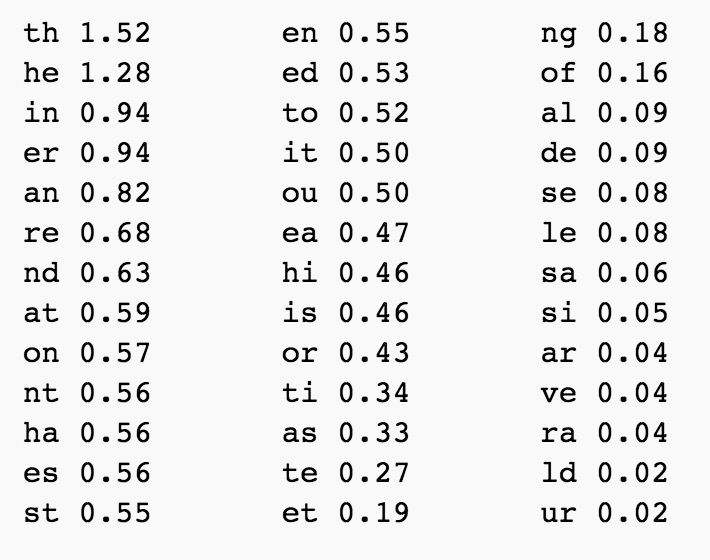
\includegraphics[width=3.5in]{Bigram.jpg}\\
	\tiny{(From \url{https://en.wikipedia.org/wiki/Bigram#Bigram_frequency_in_the_English_language}.)}
	\end{center}
	\vspace{.4in}
	\item We have a choice here.  Suppose \texttt{W} corresponds to the plaintext letter of \texttt{d}.  Since \texttt{ZRW} and \texttt{RZW} both occur at the beginning, and since \texttt{RW} occurs again later on and \textit{nd} is a common digram, let's try saying that \texttt{R} corresponds to \texttt{n}.  At this point, we have 3 letters deciphered.  What does your text look like so far?\\

{\Large\texttt{YIFQFMZRWQFYVECFMDZPCVMRZWNMDZVEJBTXCDDUMJ}}\\\vspace{.1in}

{\Large\texttt{NDIFEFMDZCDMQZKCEYFCJMYRNCWJCSZREXCHZUNMXZ}}\\\vspace{.1in}

{\Large\texttt{NZUCDRJXYYSMRTMEYIFZWDYVZVYFZUMRZCRWNZDZJJ}}\\\vspace{.1in}

{\Large\texttt{XZWGCHSMRNMDHNCMFQCHZJMXJZWIEJYUCFWDJNZDIR}}\\\vspace{.1in}

\item We can keep looking at bigrams and frequently-occurring letters to slowly fill in the rest of the letters until we get to the following message.  Can you fill in the final letters?\\


{\Large\texttt{o-r-riend-ro--arise-a-inedhise--t---ass-it}}\\\vspace{.1in}

{\Large\texttt{hs-r-riseasi-e-a-orationhadta-en--ace-hi-e}}\\\vspace{.1in}

{\Large\texttt{he-asnt-oo-in-i-o-redso-e-ore-ineandhesett}}\\\vspace{.1in}

{\Large\texttt{-ed-ac-inhischair-aceti-ted--to-ardsthes-n}}\\\vspace{.1in}


\end{enumerate}


\end{document}